\documentclass[12pt]{article}
%\usepackage{natbib}
\usepackage[french]{babel}
\usepackage{url}
\usepackage[utf8x]{inputenc}
\usepackage{graphicx}
\graphicspath{{images/}}
\usepackage{parskip}
\usepackage{fancyhdr}
\usepackage{vmargin}
\usepackage{xcolor}
\usepackage{bbm}
\usepackage{amsmath,amssymb}
\usepackage{amsthm}
\usepackage{dsfont}
\usepackage{stmaryrd}
\usepackage{systeme}
\usepackage{enumitem}
\usepackage{xcolor}
\usepackage{pifont}
\usepackage{textcomp}
\usepackage[cache=false]{minted}
\definecolor{LightGray}{gray}{0.95}
\title{Nombres algébriques et résultant}
\author{CARVAILLO T.}
\date{\today}

\makeatletter
\let\thetitle\@title
\let\theauthor\@author
\let\thedate\@date
\makeatother

\pagestyle{fancy}
\fancyhf{}
\rhead{\theauthor}
\lhead{\thetitle}
\cfoot{\thepage}
\def\dotfill#1{\cleaders\hbox to #1{.}\hfill}
\newcommand\dotline[2][.5em]{\leavevmode\hbox to #2{\dotfill{#1}\hfil}}

\newcommand{\jL}{\mathbbm{L}}
\newcommand{\Z}{\mathbbm{Z}}
\newcommand{\Q}{\mathbbm{Q}}
\newcommand{\R}{\mathbbm{R}}
\newcommand{\C}{\mathbbm{C}}
\newcommand{\K}{\mathbbm{K}}
\newcommand{\F}{\mathbbm{F}}
\newcommand{\Fq}{\mathbbm{F}_q}
\newcommand{\Fqn}{\mathbbm{F}_{q^n}}

%définition commande présentation fonction
\newcommand{\fonction}[5]{
\begin{displaymath}
\begin{array}{l|rcl}
\displaystyle
#1 : & #2 & \longrightarrow & #3 \\
    & #4 & \longmapsto & #5
\end{array}
\end{displaymath}
}
%fin définition

% de jolies accolades
\newcommand{\accolade}[2]{
\begin{displaymath}
%#1 = \left\{
    \begin{array}{ll}
       #1 %& \mbox{si }
       #2 %& \mbox{sinon.}
    \end{array}
\right.
\end{displaymath}
}
% de jolies accolades




\newtheorem{prop}{Proposition}
\newtheorem{thm}{Théorème}
\newtheorem{cor}{Corollaire}
\newtheorem{lem}{Lemme}
\theoremstyle{definition}\newtheorem{defn}{Définition}
\theoremstyle{definition}\newtheorem{exm}{Exemple}
\theoremstyle{definition}\newtheorem{rem}{Remarque}
\theoremstyle{definition}\newtheorem{algo}{Algorithme}
\theoremstyle{remark}\newtheorem{exo}{Exercice}
\theoremstyle{remark}\newtheorem{nota}{Notation}


\begin{document}

%%%%%%%%%%%%%%%%%%%%%%%%%%%%%%%%%%%%%%%%%%%%%%%%%%%%%%%%%%%%%%%%%%%%%%%%%%%%%%%%%%%%%%%%%

\begin{titlepage}
	\centering
    \vspace*{0.5 cm}
    \textsc{\LARGE Projet de Calcul Formel.\\
    \vspace{12pt}
2020-2021}\\[1.0 cm]
    \dotline[15pt]{15cm}\\
	
\includegraphics[scale = 2.2]{logo.png}
	\dotline[15pt]{15cm}\\
	\vspace{1.5cm}
	\textsc{\Large Faculté des Sciences et Techniques}\\
	\textsc{\large Master 1 - Maths. CRYPTIS}\\[1.0 cm]
	\rule{\linewidth}{0.2 mm} \\[0.4 cm]
	{ \huge \bfseries \color{blue} \thetitle}\\
	\rule{\linewidth}{0.2 mm} \\[1.5 cm]
	
	\begin{minipage}{0.4\textwidth}
		\begin{flushleft} \large
			\emph{A l'attention de :}\\
			NALDI S.\\
			\phantom{a}\\
			\phantom{a}\\
		\end{flushleft}
	\end{minipage}
	\begin{minipage}{0.5\textwidth}
    	\begin{flushright} \large
		\emph{Rédigé par :}\\
		PIARD A.\\
		JACQUET R.\\
		CARVAILLO T.\\
		\end{flushright}
	\end{minipage}\\[2 cm]
\end{titlepage}

%%%%%%%%%%%%%%%%%%%%%%%%%%%%%%%%%%%%%%%%%%%%%%%%%%%%%%%%%%%%%%%%%%%%%%%%%%%%%%%%%%%%%%%%%

\tableofcontents

%\section*{\Huge Notation}
%\vspace{3cm}
%\begin{tabular}{p{4cm}p{15cm}}
%$\mathbbm{F}_q$ & Corps de \textit{Galois} à $q$ éléments.\\
%$\mathbbm{F}_q$* & Ensemble des éléments inversibles de $\mathbbm{F}_q$\\
%\end{tabular}
%\pagebreak

%%%%%%%%%%%%%%%%%%%%%%%%%%%%%%%%%%%%%%%%%%%%%%%%%%%%%%%%%%%%%%%%%%%%%%%%%%%%%%%%%%%%%%%%%
\pagebreak
\section*{Introduction}
\addcontentsline{toc}{part}{Introduction}
\begin{figure}[h]
Lorem ipsum dolor sit amet, consectetur adipiscing elit. Donec et eleifend erat, eu aliquam elit. Etiam eu viverra est. Proin sed diam vel orci vehicula egestas. In facilisis scelerisque elit. Integer et hendrerit quam, sed pellentesque velit. Nullam pellentesque dui ac luctus rhoncus. Duis fringilla dapibus lorem in hendrerit. Duis efficitur fringilla consequat. Quisque viverra purus ac nibh tristique iaculis. Donec euismod diam sem, quis sagittis lacus volutpat sit amet. Sed nec ultricies eros. Suspendisse ullamcorper est ut sapien ultrices, in sodales massa tempus. Lorem ipsum dolor sit amet, consectetur adipiscing elit. Morbi dignissim dapibus ultrices.\\

Nunc hendrerit, erat bibendum pharetra pellentesque, risus nulla congue lorem, et lobortis libero magna quis ligula. Praesent et elementum nulla. In hac habitasse platea dictumst. Nulla dignissim nibh sodales nulla tristique condimentum. Nam luctus urna ac ligula scelerisque, non euismod ante pulvinar. Vivamus luctus tellus quis viverra laoreet. Proin vel iaculis libero. Sed tempor massa urna, non rhoncus urna pulvinar nec. Sed ut condimentum sem. Maecenas ac dolor metus. Sed eu luctus arcu.\\

Mauris tempor mauris diam, et porttitor tortor mollis sit amet. Maecenas dui neque, imperdiet egestas posuere at, ornare vitae ligula. Fusce scelerisque dictum consequat. Etiam nec tempus nisi. Morbi scelerisque sapien augue, nec placerat ex mollis id. Donec sit amet nibh ut mi condimentum malesuada. Donec sit amet felis varius, lobortis lacus vitae, bibendum justo. Curabitur lacinia lectus ac lacinia porta. Donec elit ante, pulvinar aliquam dolor ac, ullamcorper suscipit erat. Curabitur dignissim, tortor a mollis cursus, risus sapien aliquam risus, at lobortis urna tellus at lectus. Etiam in luctus nibh. Praesent maximus orci turpis, sed tincidunt mauris aliquam id. Duis eu interdum tellus. Pellentesque nibh tellus, varius eget diam ac, viverra faucibus tellus.
\end{figure}

\vfill \eject


%%%%%%%%%%%%%%%%%%%%%%%%%%%%%%%%%%%%%%%%%%%%%%%%%%%%%%%%%%%%%%%%%%%%%%%%%%%%%%%%%%%%%%%
\pagebreak 
%%%%%%%%%%%%%%%%%%%%%%%%%%%%%%%%%%%%%%%%%%%%%%%%%%%%%%%%%%%%%%%%%%%%%%%%%%%%%%%%%%%%%%%

\section{Un peu de théorie}


\subsection{Rappels}

\begin{defn}
On appelle corps tout anneau $A$ abélien unitaire dans lequel tout élément non nul est inversible, i.e. $A^{\times} = A  - \{0\}$.
\end{defn}

\begin{nota}
Dans ce qui suit, le corps de base sera noté $\K$ et désignera indifféremment, sauf indication contraire, $\Q$, $\R$ ou $\C$. 
\end{nota}

\begin{defn}
On appelle extension de $\K$ tout corps $\jL$ contenant un sous-corps isomorphe à $\K$. On notera $\jL / \K$ une telle extension.
\end{defn}

\begin{defn}
On appelle degré de l'extension $\jL / \K$ la dimension de $\jL$ en tant que $\K$-espace vectoriel. On le notera $[\jL : \K]$.
\end{defn}

\begin{prop}
Soit $E \subseteq F \subseteq G$ une tour d'extension de corps. On a alors, 
\begin{center}
$[G : E] = [G : F] \cdot [F : E]$.
\end{center}
\end{prop}

\begin{defn}
On dit que $\jL / \K$ est finie si elle est de degré finie.
\end{defn}

\begin{prop}
L'ensemble $\K[X]$ des polynômes à coefficients dans $\K$ en l'indéterminée $X$ est muni d'une structure d'anneau Euclidien.
\end{prop}


\subsection{Eléments algébriques}

\begin{defn}
Soient $\jL/\K$ une extension de corps et $P(X) = \sum_{i=0}^{n}a_iX^i$ un polynôme de degré $n$ à coefficients dans $\K$. On considère le morphisme d'évaluation \fonction{ev_\alpha}{\K[X]}{\jL}{P(X)}{P(\alpha)}
Soit $I(\alpha) :=  ker(ev_\alpha) = \{ P \in \K[X]$ tels que $P(\alpha) = 0\}$; on a deux possibilités:

\begin{itemize}
	\item Soit $I(\alpha) \ne \{ 0 \}$, i.e. $ev_a$ n'est pas injective et donc $\exists P \in \K[X] - \{0\}$ tel que $P(\alpha) = 0$. \newline
Dans ce cas $\alpha$ est dit algébrique sur $\K$.
	\item Soit $I(\alpha) = \{ 0 \}$ i.e. $ev_a$ est injective et donc $\nexists P \in \K[X] - \{0\}$ tel que $P(\alpha) = 0$. \newline
Dans ce cas, $\alpha$ est dit transcendant sur $\K$.
\end{itemize}
\end{defn}


\begin{thm}
Soit $\jL / \K$ une extension de corps et $\alpha$ un élément algébrique sur $\jL$, alors il existe un unique polynôme $P(X)$ unitaire irréductible dans $\K[X]$ vérifiant
\begin{center} ($Q(X) \in \K[X] - \{0\}$ et $Q(\alpha)=0$) ssi $P(X) \mid Q(X)$\end{center}
\end{thm}

\begin{proof}
$\K[X]$ est euclidien, donc en particulier principal. Il s'ensuit qu'il existe $P(X) \in \K[X] - \{0\}$ unitaire tel que $I(a) = (P(X))$, $I(a)$ étant un idéal propre non nul. Par le premier théorème d'isomorphisme, on obtient que $Im(ev_\alpha) \simeq \frac{\K[X]}{(P(X))}$. \newline
Ce dernier étant intègre, on obtient que $P(X)$ est premier donc irréductible dans $\K[X]$ factoriel. \newline
Il s'ensuit naturellement que $Q(X) \in I(a) - \{0\} = (P(X)) - \{0\}$ ssi $P(X) \mid Q(X)$.
\end{proof}

\begin{prop}[Admise]
On a de plus $deg(P) = [\jL : \K]$.
\end{prop}

\begin{defn}
Le polynôme $P(X)$ comme décrit ci-dessus est appellé le polynôme minimal de $\alpha$ sur $\K$ et est noté $Irr(\alpha,X,\K)$.
\end{defn}

\begin{rem}
Soit $\alpha \in \Q$, il peut être intéressant de remarquer qu'un polynôme irréductible dans $\Q[X]$ annulant $\alpha$ sera son toujours son polynôme minimal sur $\Q$. Cela découle de ce qui a été vu plus haut.
\end{rem}

\begin{prop}[Critère d'Eiseinstein - Admis]
Soit $P(X) = \displaystyle \sum_{i=0}^{n}a_iX^i$ un polynôme de $\Z[X]$. S'il existe $p$ premier tel que $\forall i \in \llbracket 0, n-1 \rrbracket$
\begin{itemize}
	\item $p \mid a_i$, 
	\item $p \nmid a_n$
	\item $p^2 \nmid a_0$
\end{itemize}
alors $P(X)$ est irréductible dans $\Q[X]$.
\end{prop}

\begin{exm}
Voyons quelques cas triviaux :
	\begin{itemize}
		\item $i$ est algébrique sur $\Q$, en effet $X^2-1$ est son polynôme minimal sur $\Q$.
		\item $\sqrt2$ et $\sqrt3$ sont algébrique sur $\Q$, de polynôme minimaux respectif $X^2 -2$ et $X^2-3$, dont l'irréductibilité découle du critère d'Eisenstein.
		\item $\alpha = \sqrt2 + \sqrt3$ est également algébrique sur $\Q$. En effet,
\begin{align*}
 \alpha = \sqrt2 + \sqrt3 &\Leftrightarrow (\alpha-\sqrt2)^2= 3\\ &\Leftrightarrow \alpha^2 + 2\alpha\sqrt2 + 2 = 3\\ &\Leftrightarrow \alpha^2 - 1 =  -2\alpha\sqrt2\\ &\Leftrightarrow \alpha^4 - 2\alpha^2 +1 =  8\alpha^2\\ &\Leftrightarrow \alpha^4 - 10\alpha^2 +1 = 0
\end{align*}		
$\alpha$ admet donc pour polynôme minimal $X^4 -10X^2 +1$. L'irréductibilité découle de Eisenstein pour $p=2$.	
	\end{itemize}
\end{exm}

\begin{defn}
Soit $\jL / \K$ une extension. On appelle fermeture algébrique de $\K$ dans $\jL$ l'ensemble des éléments de $\jL$ algébriques sur $\K$.
\end{defn}

\begin{defn}
On dit que $\jL / \K$ est algébrique si tout élément de $\jL$ est algébrique sur $\K$.
\end{defn}

\begin{prop}[Admise]
Une extension finie est algébrique.
\end{prop}

\begin{nota}
On notera $\K(\alpha_1, ..., \alpha_n)$ le plus petit corps, au sens de l'inclusion, contenant $\K$, $\alpha_1$, ..., $\alpha_n$.
\end{nota}

\begin{thm}
Soit $\jL/\K$ une extension de corps et soient $\alpha$ et $\beta$ deux éléments de $\jL$ non nuls algébriques sur $\K$. Alors, $\alpha + \beta$, $\alpha.\beta$ et $\alpha^{-1}$ sont algébriques sur $\K$. En d'autres termes, la fermeture algébrique de $\K$ est une extension de $\K$.
\end{thm}

\begin{proof}
Nous allons donner ici une première preuve non constructive. $\K(\alpha)/\K$ et $\K(\beta)/\K$ sont finies et $[\K(\alpha, \beta) : \K] = [\K(\alpha, \beta) : \K(\alpha)].[\K(\alpha) : \K]$ \newline
De plus, on a $K\subseteq \K(\alpha) \subseteq \K(\alpha,\beta)$ et $ \K\subseteq \K(\beta) \subseteq \K(\alpha,\beta)$ donc 
\begin{center}
$deg(Irr(\beta,X,\K(\alpha))) \le deg(Irr(\beta,X,\K))$
\end{center}
d'où 
\begin{center}
$[\K(\alpha,\beta) : \K] \le [\K(\beta) : \K].[\K(\alpha) : \K] < \infty$
\end{center}
Donc  $[\K(\alpha, \beta) : \K]$ est fini et l'extension est algébrique. Il s'ensuit naturellement que $\alpha + \beta$, $\alpha.\beta$ et $\alpha^{-1}$ sont algébriques, car contenus dans $\K(\alpha, \beta)$.
\end{proof}


\subsection{Résultants}

Introduisons maintenant une notion fondamentale, celle de \textit{résultant}, qui va nous permettre de donner une seconde démonstration - cette fois ci constructrice - du dernier théorème.

\begin{defn}
Soient $A = \displaystyle\sum_{i=0}^n a_iX^i$ et $B = \displaystyle\sum_{i=0}^m b_iX^i$ deux polynômes de $\K[X]$. On appelle matrice de Sylvester de $P$ et $Q$ la matrice de taille $(m+n)\times(m+n)$ définit par :
\begin{center}
$$\begin{array}{cc} 
Syl(A,B) :=
   \begin{pmatrix} 
a_n & a_{n-1} & \cdots & a_1 & a_0 & 0 & \cdots & 0 \\
0 & a_n & \cdots & a_2 & a_1	 & a_0 & \cdots & 0 \\
\vdots & \vdots & \ddots & \vdots & \vdots & \vdots & \ddots & \vdots\\
0 & 0 & \cdots & a_n & a_{n-1} & a_{n-2} & \cdots & a_0 \\
b_m & b_{m-1} & \cdots & b_1 & b_0 & 0 & \cdots & 0 \\
0 & b_m & \cdots & b_2 & b_1	 & b_0 & \cdots & 0 \\
\vdots & \vdots & \ddots & \vdots & \vdots & \vdots & \ddots & \vdots\\
0 & 0 & \cdots & b_m & b_{m-1} & b_{m-2} & \cdots & b_0 \\
   \end{pmatrix} 
&  \begin{array}{c} 
      \left. \rule{0pt}{12mm} \right\} m \\
      \left. \rule{0pt}{12mm} \right\} n 
   \end{array} 
\end{array}$$
\end{center}
\end{defn}

\begin{defn}
On appelle résultant de $A$ et $B$ le déterminant de la matrice de Sylvester de $A$ et $B$:
\begin{center} $Res(A,B) := det(Syl(A,B))$ \end{center}
\end{defn}

\begin{thm}[Admis]
Soient $A$ et $B \in \K[X]$, alors $Res(A,B) = 0$ si et seulement si $A$ et $B$ ont un facteur commun non constant dans $\K[X]$.
\end{thm}

\begin{nota}
On notera $Res_Y(A,B)$ le résultant de deux polynômes en la variable $Y$ à coefficient dans $\K[X]$.
\end{nota}

Nous allons maintenant considérer $\alpha$ et $\beta$ deux éléments de $\jL$ algébriques sur $\K$. On notera respectivement leur polynômes minimaux $A(X)$ et $B(X)$ $\in \K[X]$, avec $deg(A) = n$ et $deg(B) = m$. L'objectif est de construire un polynôme annulateur de $\alpha + \beta$, $\alpha.\beta$ et $\alpha^{-1}$ afin de donner une preuve constructive du \textit{Théorème 2}.

\begin{prop}
La fermeture algébrique de $\K$ dans $\jL$ est munie d'une structure d'anneau. En effet,
	\begin{enumerate}[label=\roman*)]
		\item Le polynôme $S(X) := Res_Y(A(Y),B(X-Y))$ est \textit{un} polynôme annulateur de $\alpha + \beta$.
		\item Le polynôme $P(X) := Res_Y(A(Y), X^m.B(\frac{X}{Y}))$ est \textit{un} polynôme annulateur de $\alpha.\beta$.
	\end{enumerate}
\end{prop}
\begin{proof} De simples calculs suffisent, remarquons que
	\begin{enumerate}[label=\roman*)]
		\item $S(\alpha + \beta) = Res_Y(A(Y),B(\alpha + \beta - Y))$. Or, $A(\alpha) = 0$ et $B (\alpha-\alpha + \beta) = B(\beta) = 0$. Donc les polynômes $A(Y)$ et $B (\alpha + \beta - Y) \in \K[Y]$ admettent $\alpha$ comme racine commune. De part le théorème précédent, on obtient que $S(\alpha + \beta) = Res_Y(A(Y),B(\alpha + \beta-Y)) = 0$, la conclusion s'ensuit. 
		\item De manière similaire, $P(\alpha.\beta) = Res_Y(A(Y), (\alpha.\beta)^m.B(\frac{\alpha.\beta}{Y}))$. Or, $A(\alpha) = 0$ et $(\alpha.\beta)^m.B(\frac{\alpha.\beta}{\alpha}) = (\alpha.\beta)^m.B(\beta) = 0$ Le terme $(\alpha.\beta)^m$ est nécessaire lorsque $\alpha = 0$. La conclusion s'ensuit.
	\end{enumerate}
\end{proof}
\begin{minted}
[
frame=lines,
framesep=2mm,
baselinestretch=1.2,
bgcolor=LightGray,
fontsize=\footnotesize,
linenos
]
{python}
# Fonction qui permet le calcul d'un polynôme annulateur
# de la somme de nombres algébriques

annulSomme := proc(u, v) 
local f, g, A, B, syl, res; 
A := PolynomialTools:-MinimalPolynomial(u, X); 
B := PolynomialTools:-MinimalPolynomial(v, X); 
f := Y -> subs(X = Y, A); 
g := Y -> subs(X = Y, B); 
syl := SylvesterMatrix(f(Y), g(Y - X), Y); 
res := Determinant(syl); 
return res; 
end proc:

# Fonction qui permet le calcul d'un polynôme annulateur
# du produit de nombres algébriques

annulProduit := proc(u, v) \\
local f, g, A, B, res, m; 
A := PolynomialTools:-MinimalPolynomial(u, X); 
B := PolynomialTools:-MinimalPolynomial(v, X); 
f := Y -> subs(X = Y, A); 
g := Y -> subs(X = Y, B); 
m := degree(g(Y)); 
res := resultant(f(Y), X^m*g(Y/X), Y); 
return res;
end proc
\end{minted}

Il vient alors la proposition suivante,
\begin{prop}
La fermeture algébrique de $\K$ dans $\jL$ est munie d'une structure de corps; en effet le polynôme $P(X) := X^n.A(1/X)$ est un polynôme annulateur de $\alpha^{-1}$.
\end{prop}

\begin{proof}
Une fois de plus, un simple calcul suffit: \newline
$P(\alpha^{-1}) = ((\alpha^{-1})^n).A(\alpha^{-1}) = \alpha^{-n}.\displaystyle\sum_{i=0}^n (\frac{a_i}{\alpha^{-1}})^i = \alpha^{-n}.\sum_{i=0}^n \alpha^i.a_i = \alpha^{-n}.P(\alpha) = 0$
\end{proof}

\begin{minted}
[
frame=lines,
framesep=2mm,
baselinestretch=1.2,
bgcolor=LightGray,
fontsize=\footnotesize,
linenos
]
{python}
# Fonction qui permet le calcul d'un polynôme annulateur
# de l'inverse d'un nombre algébrique

annulInverse := proc(u) 
local A, n, G, v; 
v := 1/u; 
A := PolynomialTools:-MinimalPolynomial(v, X); 
n := degree(A(X)); 
G := X -> X^n*A(X); 
return G(v); 
end proc

\end{minted}

\begin{exm}
Nous avons précédemment vu que le polynôme minimal de $\alpha = \sqrt2 + \sqrt3$ est $X^4 -10X^2 +1$. Retrouvons ce résultat grâce à la théorie des résultants. Soient $A$ et $B$ les polynômes minimaux de $\sqrt2$ et $\sqrt3$. Construisons $Syl(A(Y), B(Y-X))$. On a $B(Y-X) = (Y-X)^2 -3 = Y^2 + (-2X)Y + (X^2+3)$ d'où

\begin{center}
$Syl(A(Y), B(Y-X)) =$
$
   \begin{pmatrix} 
1 & 0 & -2 & 0 \\
0 & 1 & 0 & -2 \\
1 & -2X & X^2 +3 & 0 \\
0 & 1 & -2X & X^2 +3 \\
   \end{pmatrix} 
$
\end{center}

et donc,
			\begin{align*} 
Res_Y((A(Y), B(Y-X))&= \begin{vmatrix} 1 & 0 & -2 & 0 \\ 0 & 1 & 0 & -2 \\ 1 & -2X & X^2 - 3 & 0 \\ 0 & 1 & -2X & X^2 -3 \\\end{vmatrix}
			\end{align*} 
			
En utilisant la fonction Maple codée précédemment on obtient alors

\begin{figure}[h]
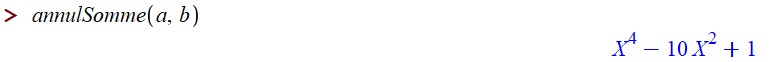
\includegraphics[scale=0.65]{code0.png}
\end{figure}

D'où $Res_Y((A(Y), B(Y-X)) = X^4 - 10X^2 + 1$.
\pagebreak

Ce qui correspond au polynôme minimal trouvé lors du précédent exemple. Nous avons ici obtenu un polynôme annulateur qui est \textit{le} polynôme minimal, mais ce ne sera pas  le cas.
\end{exm}

\section{Digression sur les corps finis}

On va ici s'intéresser au cas particulier des corps finis.

\begin{nota}
On dénotera par $q := p^n$ la puissance n-ième d'un nombre premier $p$.
\end{nota}

\begin{prop}
Pour tout $p$ premier, il existe un corps fini à $p^n$ éléments, unique à isomorphisme près, qui sera noté $\Fq$.
\end{prop}

Contrairement au cas où le corps plancher est $\Q$, nous disposons d'algorithmes de construction de polynômes minimaux efficace. 

\begin{prop}
Soient $P$ un polynôme de degré $n$ à coefficients dans $\Fq$, et $\alpha$ une racine de $P$ dans $\Fqn$. Alors $P$ admet $n$ racines (distinctes !) dans $\Fqn$, qui ne sont autre que les $\alpha^{q^i}$, où $i$ décrit $\{1, ..., n-1\}$.
\end{prop}

\begin{defn}
Soit $\alpha$ un élément algébrique de degré $n$ sur $\Fq$. On appelle conjugués de $\alpha$ sur $\Fqn$ les racines de son polynôme minimal, i.e. les $\alpha^{q^i}$, où $i$ décrit $\{1, ..., n-1\}$.
\end{defn}

Il nous est maintenant facile de constuire le polynôme minimal (dans $\Fqn$ !) de $\alpha \in \Fq$.

\begin{algo}[Méthode des conjugués]
Soit $\alpha \in \Fqn$, on calcule les puissances successive de $\alpha^{q}$ jusqu'à trouver le plus petit entier $m$ tel que $\alpha^{q^m} = \alpha$. On obtient ainsi que $\alpha$ est algébrique de degré $m$ et 
\begin{center} $Irr(\alpha, \Fq, X) = \displaystyle \prod_{i=0}^m (X-\alpha^{q^i})$. \end{center}
\end{algo}






%%%%%%%%%%%%%%%%%%%%%%%%%%%%%%%%%%%%%%%%%%%%%%%%%%%%%%%%%%%%%%%%%%%%%%%%%%%%%%%%%%%%%%%
\pagebreak
%%%%%%%%%%%%%%%%%%%%%%%%%%%%%%%%%%%%%%%%%%%%%%%%%%%%%%%%%%%%%%%%%%%%%%%%%%%%%%%%%%%%%%%

%\addcontentsline{toc}{part}{Références}

%\begin{thebibliography}{9}
	%\bibitem{these1}
	%Référence 1
%\end{thebibliography}

\end{document}
